%\documentclass[aps,prd,nofootinbib]{revtex4-1}
\documentclass[singlepage,notitlepage,nofootinbib,11pt]{revtex4-1}
\usepackage{amsmath}
\usepackage{amssymb}
\usepackage{graphicx}
\usepackage{subfig}
\usepackage{epsfig}
\usepackage{listings}
\usepackage[hidelinks,hyperfootnotes=false,bookmarks=false,colorlinks=true]{hyperref}

\newcommand{\eq}[1]{\begin{align*}#1\end{align*}}
\newcommand{\pmat}[1]{\begin{pmatrix}#1\end{pmatrix}}
\newcommand{\center}[1]{\begin{center}#1\end{center}}
\def\<{\langle}
\def\>{\rangle}
\def\l{\left}
\def\r{\right}

\begin{document}
\title{Final Exam - G6080}
\author{Victor Genty}
\email{vgenty@nevis.columbia.edu}
\homepage{www.nevis.columbia.edu/~vgenty}
\date{\today}
\begin{abstract}
\centering
Source code can be found at \href{https://github.com/vgenty/G6080/tree/master/final}{github.com/vgenty/G6080/final}
\end{abstract}
\maketitle
\section*{Introduction}
I programmed the time evolution of a quantum state obeying the schrodinger equation in C++ with the \texttt{eigen3} matrix library, and the \texttt{ROOT} data package for storing, retieving, and displaying data from the compiled program. In the instances where the compiled code needed to be executed with varying input parameters, python was used in combination with the \texttt{subprocess32} module.\\
\indent For this analysis I used the following hardcoded parameters which define the support for the 1D Schrodinger. I chose parameters which were a good balance between precision, compilation, and executation time.
\begin{center}
  \begin{tabular}{| l | c |}\hline
    Lattice $a$ & 0.0005 \\\hline
    Length $L$  & 2 \\\hline
    Lattice points $N$ & 4000\\ \hline
    Total Time $T$ & 1000 \\ \hline
    Time step $dt$ & 0.0001 \\ \hline
    \end{tabular}
\end{center}
\indent\indent A breakdown of the essential functions can be found in the last section of this paper under ``Code''.
\section*{1.1 Setup}
\begin{enumerate}
\item The updating scheme in Eq. (2) is unitary because it preserves the integral squared norm of the state vector in time i.e.
  \begin{align*}
    \int_{\mathbb{R}} dx \left|\phi(t+\Delta t)\right|^2 = \int_{\mathbb{R}} dx \left|\phi(t)\right|^2.
  \end{align*}
  Therefore it's sufficient to check if the updating scheme is norm preserving at $n+1$ and $n$. So,
  \begin{align*}
    \left|\phi^{(n+1)}\right|^2 &= \left|\frac{1-i H \Delta t/2}{1+i H \Delta t/2}\right|\left|\phi^{n}\right|^2 \\
    &= \frac{1-i H \Delta t/2}{1+i H \Delta t/2}\cdot\frac{1+i H^{\dagger} \Delta t/2}{1-i H^{\dagger} \Delta t/2}.
  \end{align*}
  Now the Hamiltonian is hermitian, $H = H^{\dagger}$ so,
  \begin{align*}
    \frac{1-i H \Delta t/2}{1+i H \Delta t/2}\cdot\frac{1+i H \Delta t/2}{1-i H \Delta t/2} &=  1,\\
  \end{align*}
  as the numerator and denominator cancel leaving,
  \begin{align*}
    \left|\phi^{n+1}\right|^2 = \left|\phi^n\right|^2.
  \end{align*}
  Therefore the updaing scheme is unitary.
\item The Schrodinger equation and be nondimensionalized with the substitutions,
  \begin{align*}
    \widetilde{\phi}&=\phi\sqrt{\frac{\hbar}{m c}}\\
    \widetilde{x}&=x\left(\frac{mc}{\hbar\right)}\\
    \widetilde{t}&=t\left(\frac{mc^2}{\hbar}\right)\\
    \widetilde{V}&=V\left(\frac{1}{mc^2}\right),
  \end{align*}
  leaving the Schrodinger equation as,
  \begin{align*}
    -\frac{1}{2}\frac{\partial^2}{\partial\widetilde{x}^2}\widetilde{\phi}+\widetilde{V}\widetilde{\phi} = i \frac{\partial}{\partial\widetilde{t}}\widetilde{\psi}.
  \end{align*}
  This gives the updating scheme the following form,
  \eq{
    \chi_{j+1}^{(n)}+\left(-2+\frac{4i\widetilde{\epsilon}^2}{\Delta\widetilde{t}}-2\widetilde{\epsilon}^2\widetilde{V_j}\right)\chi_j^{(n)} + \chi_{j-1}^{(n)} = \frac{8i\widetilde{\epsilon}^2}{\Delta\widetilde{t}}\phi_j^{(n)}.
  }
  The total range of the simulation is fixed to $-1 < x < 1$. We also set the mass $m$ equal to 1.
\end{enumerate}
\section*{1.2 Evolution of a wavepacket}
We start with a normalized gaussian wave packet at $t=0$,
\eq{
\phi(x,t=0) = \frac{1}{\sqrt{\sigma \sqrt{\pi}}}\exp\left(ikx\right)\exp\left(-(x-x_0)^2/\left(2\sigma^2\right)\right).
}
This particular wave packet has a fixed expecation energy value given by,
\begin{align*}
  \<E\> &= \<\phi|E|\phi\> = \<\phi|\frac{p^2}{2m}|\phi\> = \int_{\mathbb{R}}dx\<\phi|x\>\left(-\frac{\hbar^2}{2m}\right)\frac{\partial^2}{\partial x^2}\<x|\phi\> \\
  &= \frac{p^2}{2m} + \frac{\hbar^2}{2 m \sigma^2},
\end{align*}
and with our choice of units is
\eq{
\<E\> = \frac{k^2}{2} +  \frac{1}{4\sigma^2}.
}
Rearranging we can choose the input momentum based on the given energy,
\eq{
k = \sqrt{2 E - \frac{1}{2\sigma^2}}
  }
I checked my implementation of the algorithm, specifically my implementation of the LU factorization of the tridiagonal matrix. I evolved the free particle for a total time step of 1000, 500 steps in the forward direction then fliping the sign of the time step $dt$ and then evolving 499 steps in the reverse direction to check for unitarity. Snapshots of the wavepackets are shown in Fig. \ref{evolution}. The wavepackets are nearly identical before and after the evolution. As the gaussian propogates it spreads out in position as epected from a free particle. The elongated wave at $t=T/2$ then begins narrowing as the algorithm is reversed. We check the unitarity of the state as a function of time and plot in Fig. \ref{unitarity}. The unitarity of the state does not deviate from one out of IEEE double precision during the duration of the test simulation indicating fantastic conserved unitarity.
\begin{figure}[h]
  \centering
  \captionsetup[subfigure]{labelformat=empty}
  \subfloat[][]{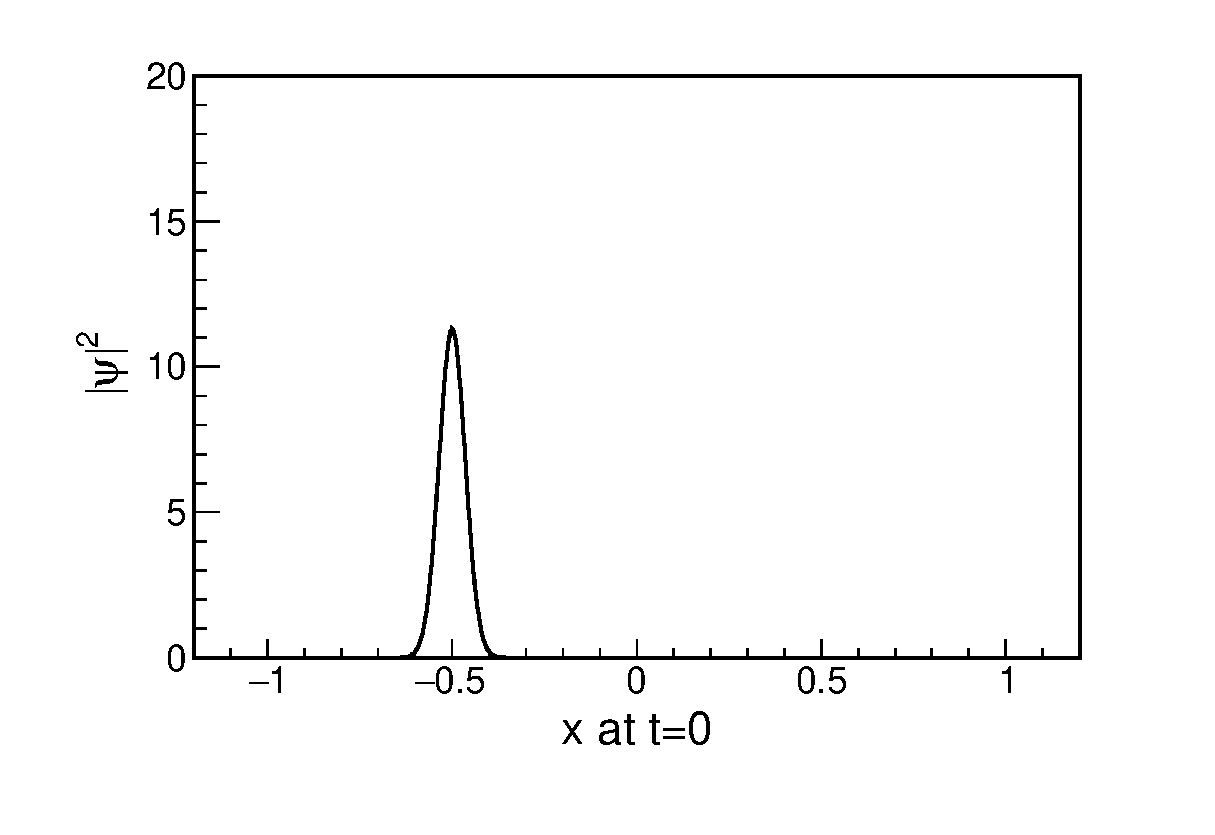
\includegraphics[width=0.5\textwidth]{figures/packet_t0.eps}}
  \subfloat[][]{\includegraphics[width=0.5\textwidth]{figures/packet_t846.eps}}\\
  \subfloat[][]{\includegraphics[width=0.5\textwidth]{figures/packet_t999.eps}}
  \caption{\label{evolution} Position space snap-shots of the specified gaussian wavepacket at three different time slices. The top left pane shows the initial state at $t=0$. The top right pane shows the impact of the gaussian wave packet with the infinite wall in reversed time. The bottom pane shows the state returning to its initial configuration.}
\end{figure}
\begin{figure}[h]
  \centering
  \captionsetup[subfigure]{labelformat=empty}
  \subfloat[][]{\includegraphics[width=0.5\textwidth]{figures/unitarity.eps}}
  \caption{\label{unitarity} Integral norm squared of gaussian wave packet as a function of time. }
\end{figure}
\clearpage
\section*{1.3 Scattering from a step function potential}
We scatter wavepackets of varying widths and incident energies at step potentials. For this problem we must ensure the wavepacket is sufficiently localized and therefore energetic enough to quickly scatter off the step potential without encountering effects from hitting the infinite walls. In Fig. \ref{EoverV} I plot the reflection and transmission coefficient for two fixed step potentials as a function of incoming energy at fixed width $\sigma=0.05$ (essentially the varying the average wavenumber $k$). A smooth rise of the transmission and corresponding lull of the of the reflection coefficient is observed for increasing energy. This result is different than for discrete incoming plane waves with fixed wavenumber. The quantum wave train softens the edge between at the classically allowed turning point which is expected as the wavepacket contains a distribution of wavenumbers based on it's width. Doubling the potential only had the effect of increasing the curvature of the reflection and transmission lines. For sufficiently high $V$ and $E$ I believe the curves would become even sharper. Next I examine the two coefficients as a function of initial gaussian width in Fig. \ref{sigmas}. The wider the initial wavepacket the more defined the incoming value for the wavenumber since $k\propto 1/\sigma$. In Fig. \ref{sigmas} the reflection and transmission coefficients approach their analytical plane wave values asymptotically for $E>V$ stated without proof,
\begin{align*}
T &= \frac{4 k_1 k_2 }{(k_1 + k_2)^2}\\
R &= \frac{(k_1 - k_2)^2}{(k_1+k_2)^2},
\end{align*}
with,
\begin{align*}
k_1 &= \sqrt{2E}\\
k_2 &= \sqrt{2(E-V)},
\end{align*}
in our dimensionless units $\hbar=c=1$ and $m=1$ for incoming plane waves with definite momentum. I chose fixed energy $E=1.25V\cdotV$ and observed that increasing the width of the wavepacket forced the coeffiecients to their plane wave values of,
\begin{align*}
T&=0.854\\
R&=0.146.
\end{align*}
Varying the size of the step potential did not appear to have any effect on the aymptotic behavior.
\begin{figure}[h]
  \centering
  \captionsetup[subfigure]{labelformat=empty}
  \subfloat[][]{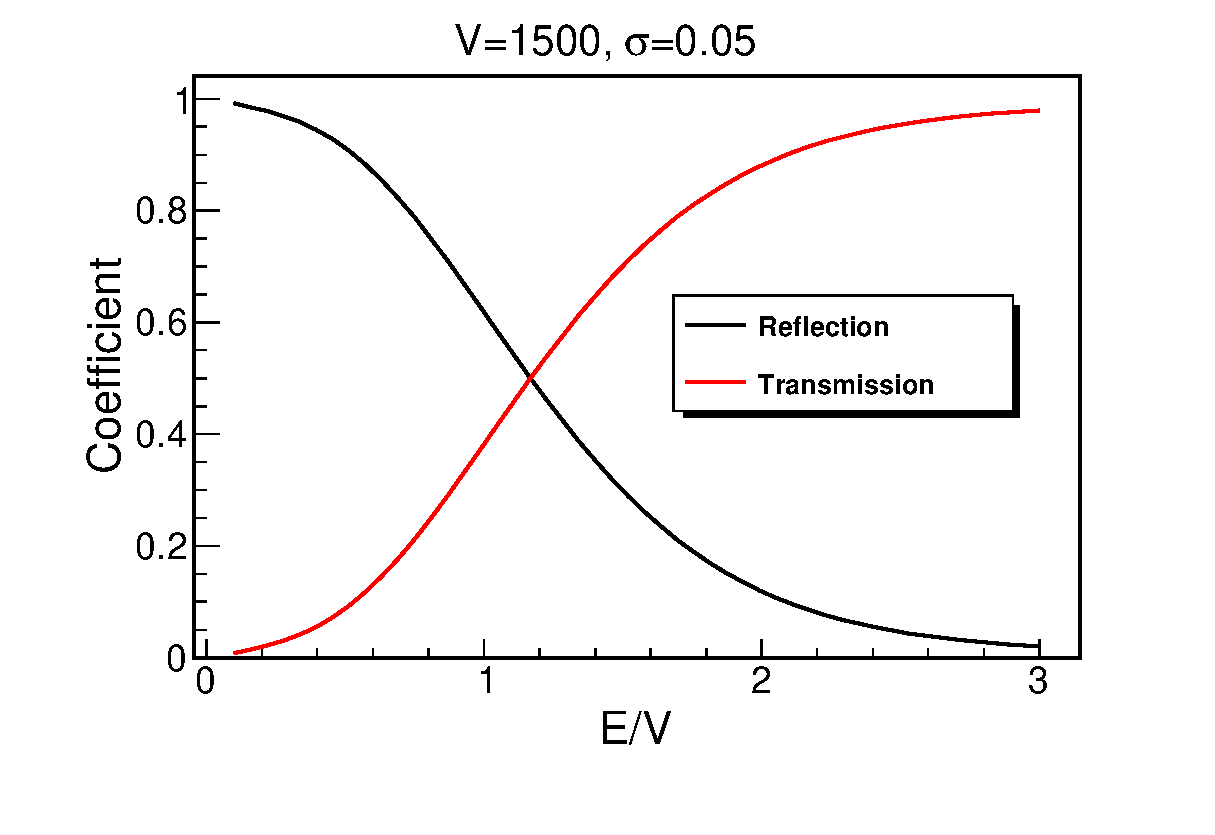
\includegraphics[width=0.5\textwidth]{figures/RT_V1500_sigma0p05.eps}}
  \subfloat[][]{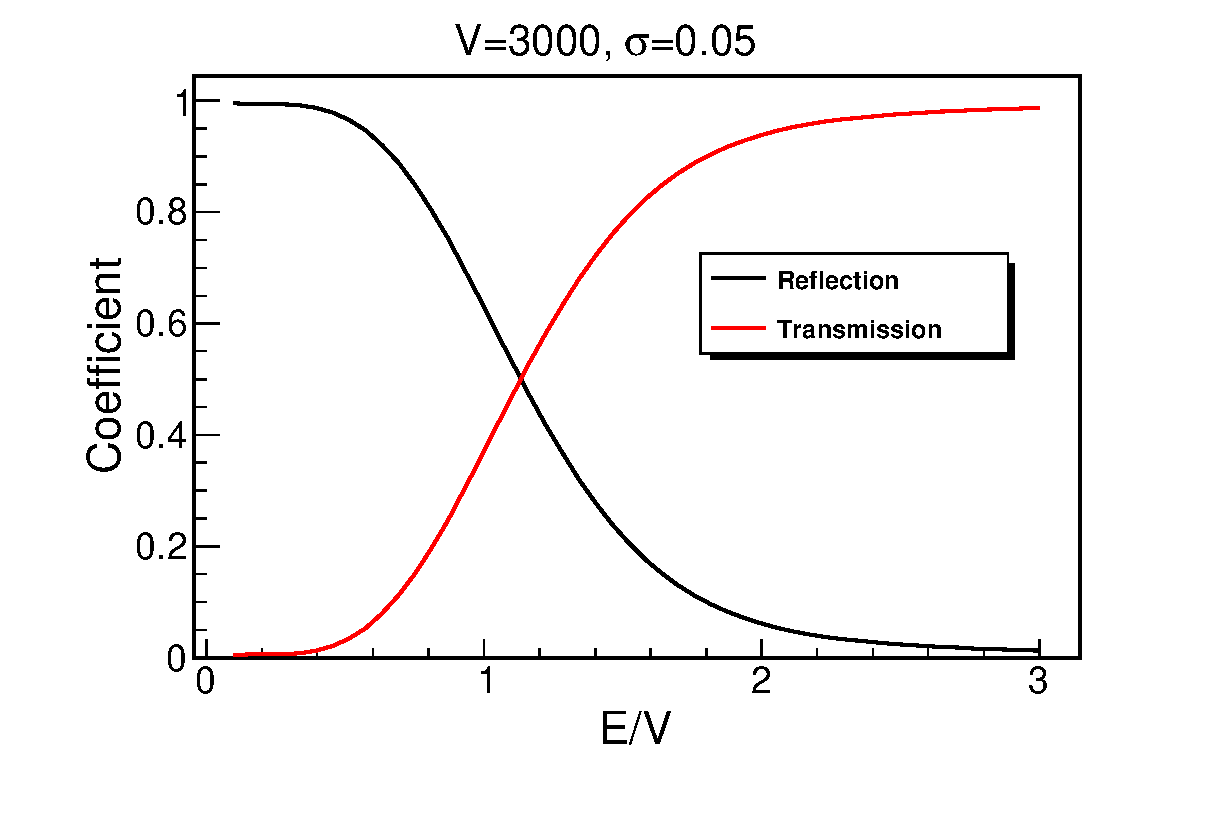
\includegraphics[width=0.5\textwidth]{figures/RT_V3000_sigma0p05.eps}}
  \caption{\label{EoverV} Reflection (black) and transmission (red) as a function of incoming energy for two different sizes of step potential. The rise in potential did not appear to have a significant effect on the transmission and reflection curves.}
\end{figure}
\begin{figure}[h]
  \centering
  \captionsetup[subfigure]{labelformat=empty}
  \subfloat[][]{\includegraphics[width=0.5\textwidth]{figures/RT_V1500_E=1p25V_sigma.eps}}
  \subfloat[][]{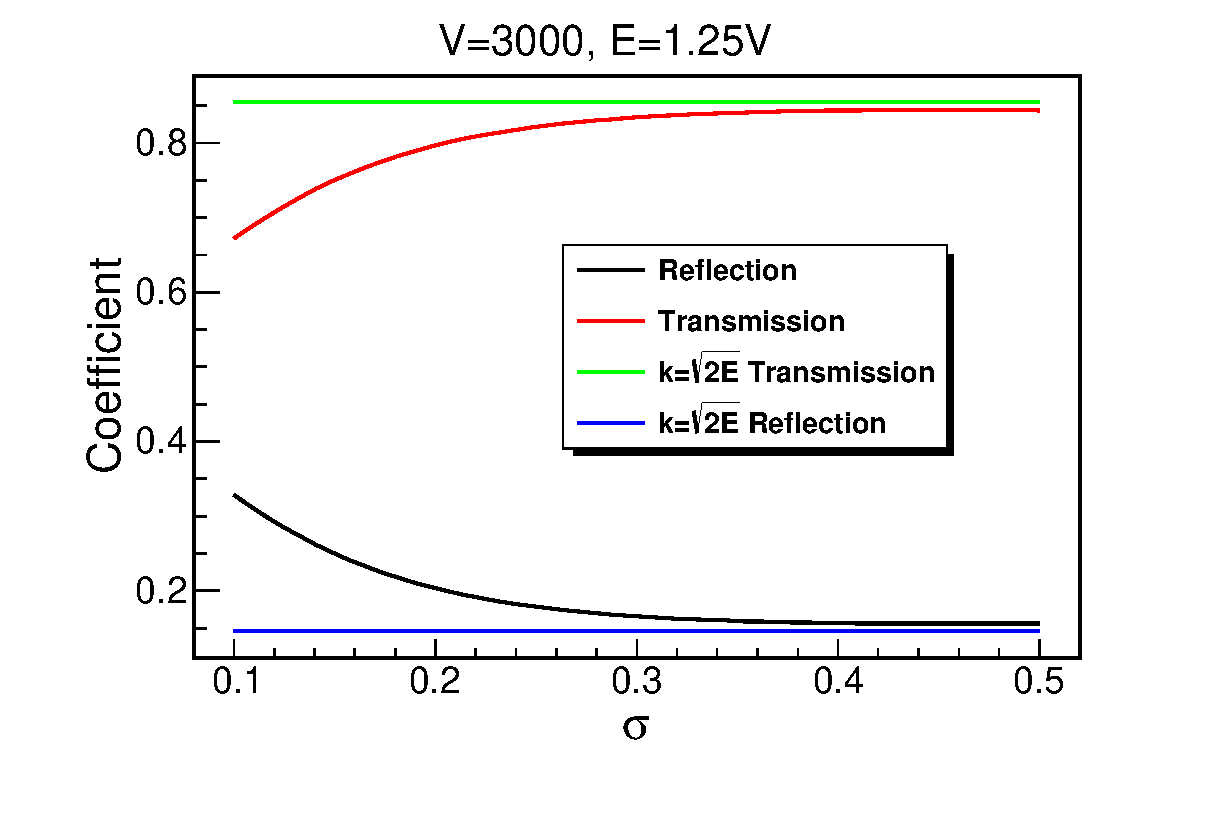
\includegraphics[width=0.5\textwidth]{figures/RT_V3000_E=1p25V_sigma.eps}}
  \caption{\label{sigmas} Reflection and transmission coefficient as a function of initial $t=0$ width of the gaussian packet. Increasing he initial width expands the gaussian packet more closely mirroring an incoming plane wave.}
\end{figure}








\clearpage
\section*{1.4 Decay of an unstable state}
We set up the quantum well potential as shown in the diagram. We start with the ground and the first excited state wavefunction in an eigenstate of an infinite well,
\begin{align*}
  \phi_{\text{ground}} &= \sqrt{\frac{2}{w}}\cos\left(\frac{\pi}{w}x)\\
  \phi_{\text{1st excited}} &= \sqrt{\frac{2}{w}}\sin\left(\frac{2\pi}{w}x)
\end{align*}
with energy,
\begin{align*}
  E_{\text{ground}} &= \frac{\pi^2}{2 w^2}\\
  E_{\text{1st excited}} &= \frac{2 \pi^2}{w^2},
\end{align*}
in our dimensionless units ($m=1$). For this simulation we set $w=0.1$, $s=0.01$, $b=0.50$, $h=3000.0$, and center the basin around $x=0$. The initial wave functions and the wavefunctions during the decay is plotted in Fig. \ref{decaying}. The initial ground state energy of the wave function $E_{\text{ground}}\approx494$ and of the first excited state $E_{\text{1st excited}}\approx 1976$ using the equation above. We then plot the probability for the particle to be found in the well as a function of time and fit the data points before the leaked probability reflects from the wall. The results are shown in Fig. \ref{expoo}. The {\it lower} the energy the state inside the well, the {\it larger} the time constant or the longer is takes for the state to diffuse outside the well. In both plots I restricted the fit region to only include the decay before the particle reflected from the infinite walls.
\begin{figure}[h]
  \centering
  \captionsetup[subfigure]{labelformat=empty}
  \subfloat[][]{\includegraphics[width=0.5\textwidth]{figures/falloff0.eps}}
  \subfloat[][]{\includegraphics[width=0.5\textwidth]{figures/falloff222.eps}}\\
  \subfloat[][]{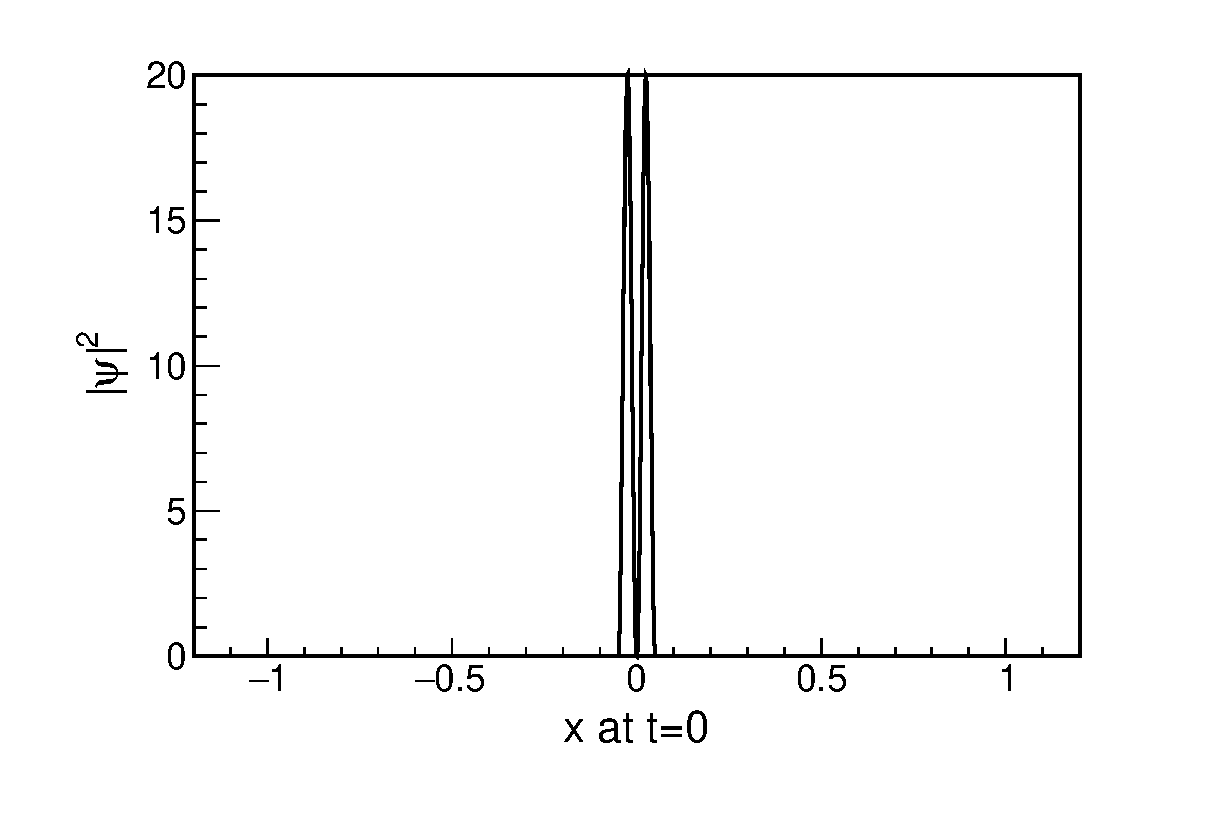
\includegraphics[width=0.5\textwidth]{figures/falloff0_sin.eps}}
  \subfloat[][]{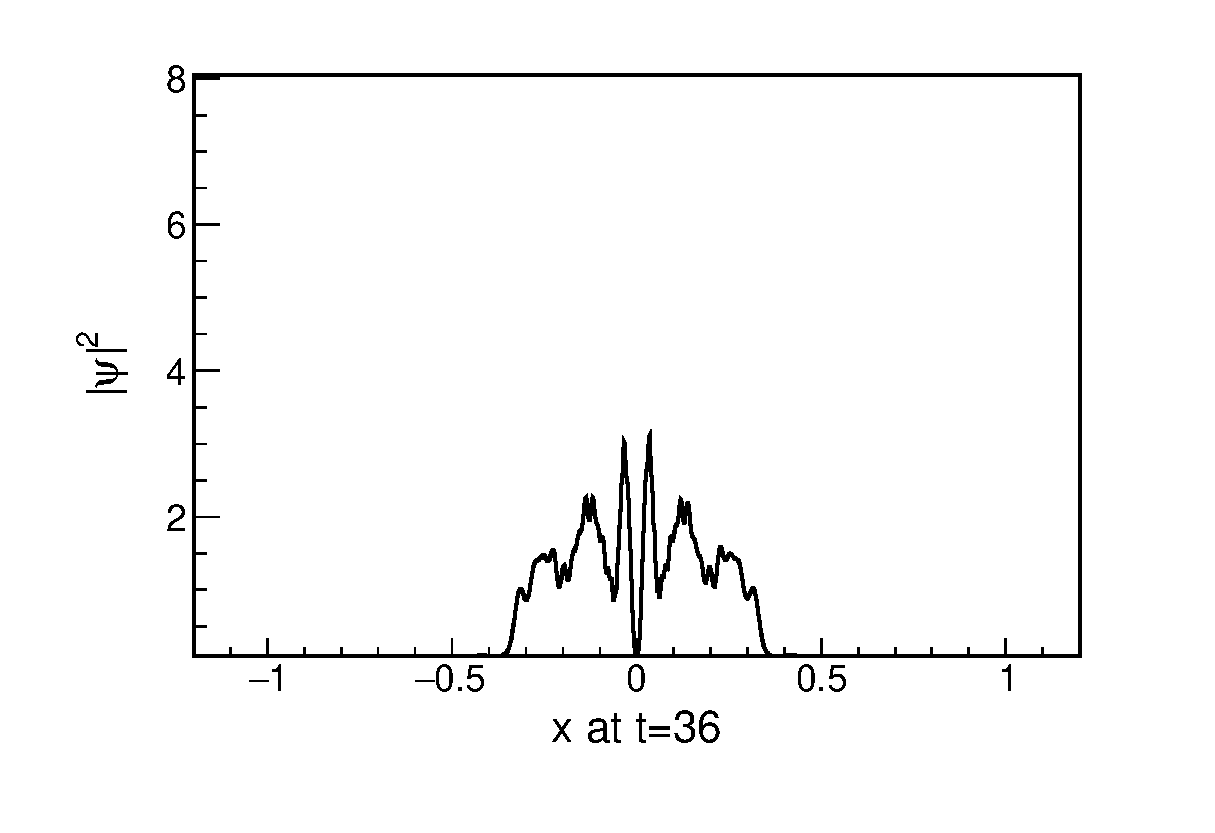
\includegraphics[width=0.5\textwidth]{figures/falloff35_sin.eps}}
  \caption{\label{decaying} The probability for the ground and first excited state density diffuses out of the confined region. The left plots show the initial configuration. The right plots shows the state during is exponential decay as it penetrates with classically unallowed region.}
\end{figure}

\begin{figure}[h]
  \centering
  \captionsetup[subfigure]{labelformat=empty}
  \subfloat[][]{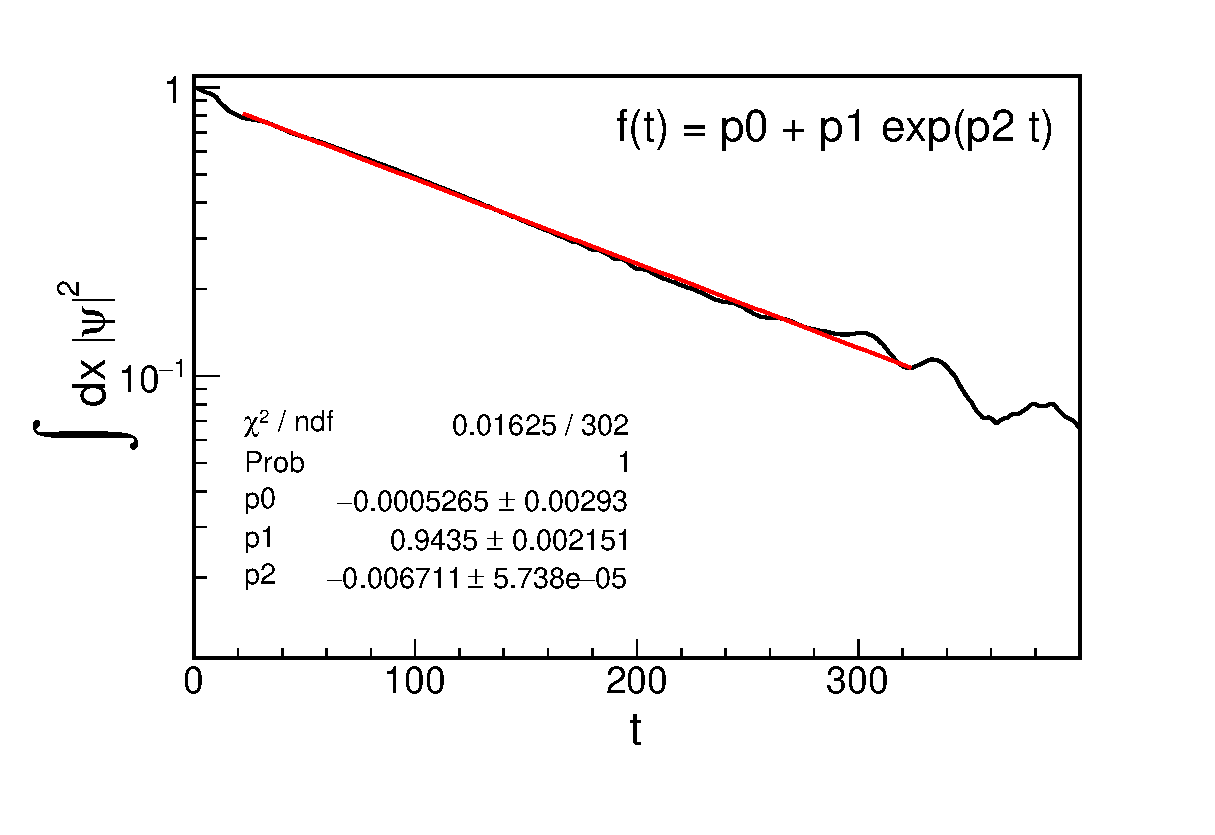
\includegraphics[width=0.5\textwidth]{figures/expo_decay.eps}}
    \subfloat[][]{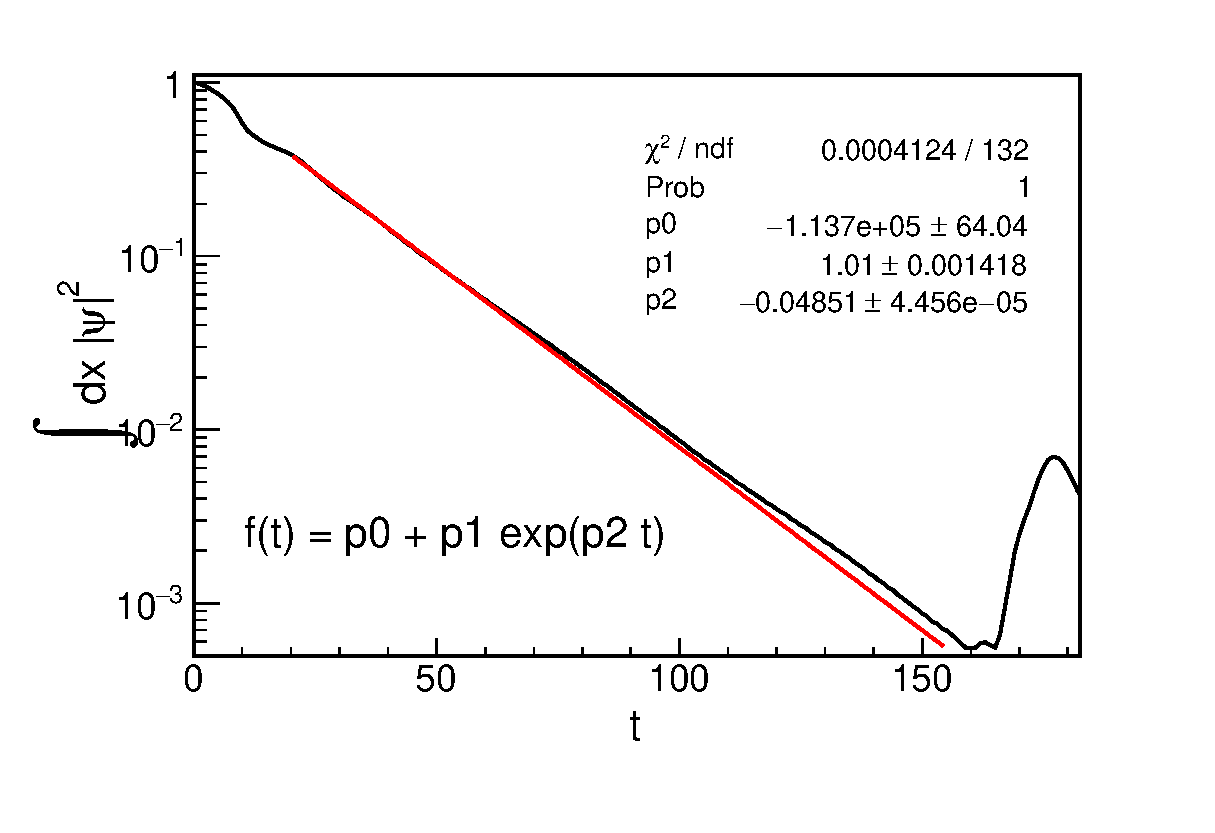
\includegraphics[width=0.5\textwidth]{figures/expo_decay_sin.eps}}
  \caption{\label{expoo} {\it Left plot:} ground state. {\it Right plot:} first excited state. Exponential decay of the probability density inside the well or ``resonance''. The log plot above shows the red line fit via the \texttt{MINUIT} fit package. The decay constant is $1/\texttt{p2}\approx150} for the ground state and $1/\texttt{p2}\approx20$ for the first excited state.}
\end{figure}
\clearpage
\section*{1.5 Scattering G6080}
We now consider scattering from this potential in the previous problem. I sent in wave packet to scatter the potential in the previous problem with varying energies. The result is plotten in Fig. \ref{resonance}. Peaks in the spectrum occur on intervals {\it spaced quadratically} mirroring the energy splitting between the levels of the infinite well potential. Even more interesting is that these energies correspond the energies of the infinite well of width $w$! The time evolution for a particle passing through the double potential eith $E<V_{\text{side}}$ is shown in Fig. \ref{evo}. I spaced out the side of the well to show the salient features which are the following. The initial particle passes through the first wall, a some of the wave reflects, some makes it through, it continues propogation to the second wall and less of the amplitude crosses while most reflects. At a finite time later the probability mass takes on the structure of a high energy eigenstate of the infinite well.
\begin{figure}[h]
  \centering
  \captionsetup[subfigure]{labelformat=empty}
  \subfloat[][]{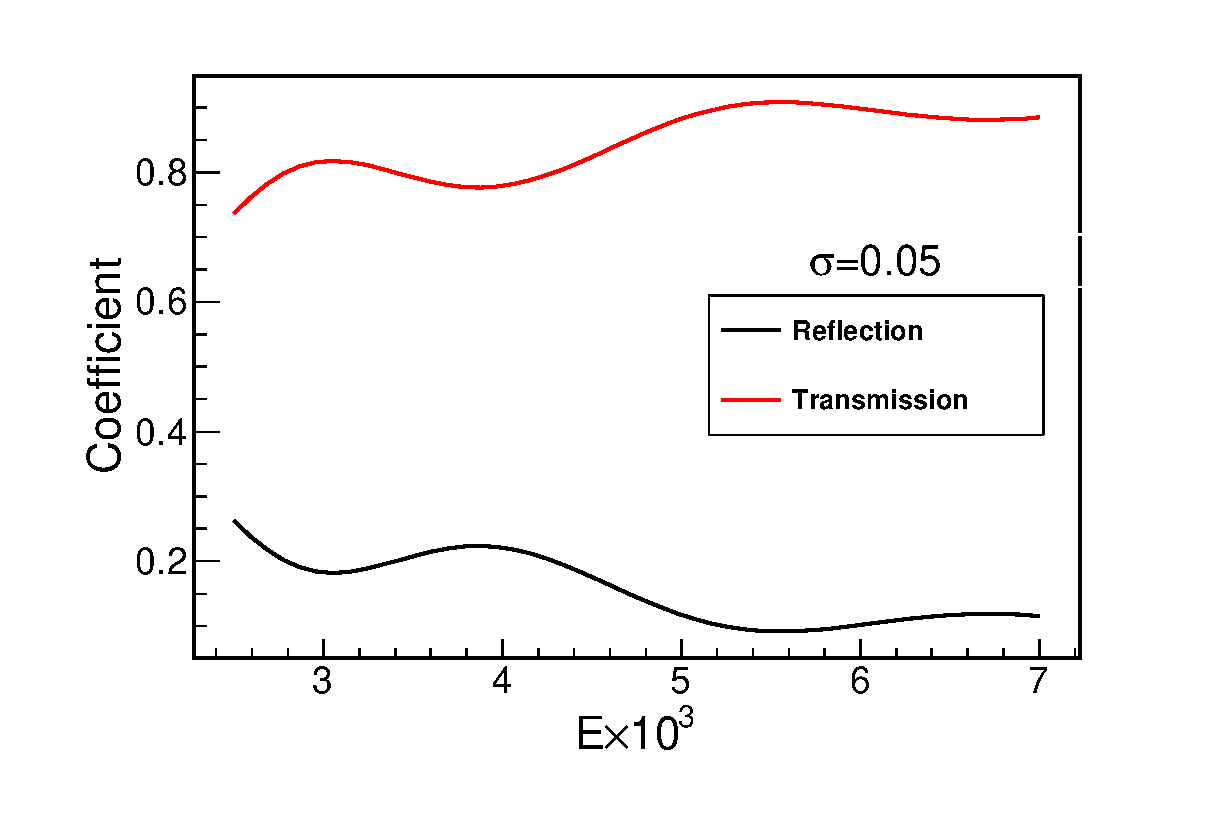
\includegraphics[width=0.5\textwidth]{figures/resonance.eps}}
  \caption{\label{resonance} Transmission and reflection spectrum as a function of incoming energy. For $E>3000.0$ (the maximum of the well) resonance is observed.}
\end{figure}
\begin{figure}[h]
  \centering
  \captionsetup[subfigure]{labelformat=empty}
  \subfloat[][]{\includegraphics[width=0.333\textwidth]{figures/t0.eps}}
  \subfloat[][]{\includegraphics[width=0.333\textwidth]{figures/t32.eps}}
  \subfloat[][]{\includegraphics[width=0.333\textwidth]{figures/t71.eps}}\\
  \subfloat[][]{\includegraphics[width=0.333\textwidth]{figures/t107.eps}}
  \subfloat[][]{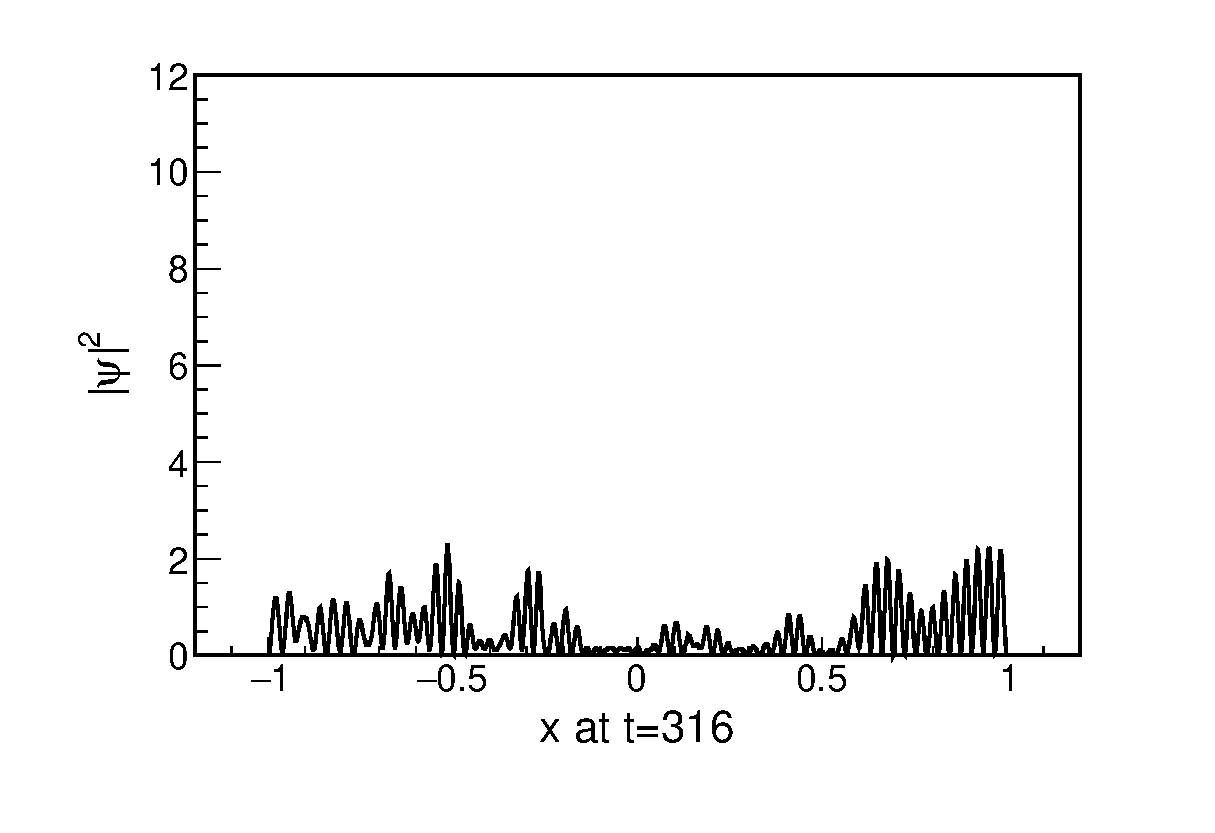
\includegraphics[width=0.333\textwidth]{figures/t316.eps}}
  \caption{\label{evo} Time evolution of the particle as it crosses the double barrier for $E<V$.}
\end{figure}
\clearpage
\section*{Code}
The main program is called \texttt{evolve.cpp} which can be build with the provided \texttt{Makefile}. The flow chart is as follows
\begin{center}{\bf \texttt{evolve.cpp}}\end{center}
\begin{enumerate}
\item  The first part of the program gives parameters definitions for the simulations such as $a$, $L$, $N$, etc. The output stream to the \texttt{ROOT} file is also initialized.
\item The lattice is set up as an \texttt{std::vector<double>} and an initial wavefunction can be defined.
\item Next the ``sparse'' tri-diagonal matrix \texttt{W} is built with the recursion schemedm defined in the problem. The boundary conditions are defined in this matrix by placing $psi=0$ on the upper left and bottom right of this matrix. The sparse matrix class provided by \texttt{eigen3} only stores the non-zero entries of the matrix providing for light and quick access. The \texttt{W} matrix is also outfitted with the specified potential energy distribution.
\item The \texttt{W} matrix is factorized via LU decomposition in the\\ \texttt{get\_LU(SparseMatrix<std::complex<double> >)} method.
\item For the specified time interval a for loop solves the LU equation with the function \texttt{solve\_LU}. I took inspiration for this algorithm from the Numerical Recipies book and notes from class. The solution vector is stored in an STL vector as \texttt{std::vector<VectorXcd>}.
  \item Finally, a for each function with a lambda expression access the contents of the solution vector each time step and ``Fill()''s the \texttt{ROOT} tree and the simulation completes.
\end{enumerate}
Various other python scripts are included which essentially just help visualize the output of the simulation:
\begin{itemize}
\item \texttt{plotter.py} - Visualized the norm squared distribution of the state as a function of time. Takes a ROOT file as an input.
\item \texttt{unitarity.py} - Check unitarity as a function of time.
\item \texttt{decay.py} - Plot the probability of being in the well as a funtion of step.
\item \texttt{j.py} - Plot the reflection and transmission coefficients as a function of energy. This script executes the C++ main program for different initial energies and plots the $R$ and $T$ as a function of $E/V$. Used for barrier scattering.
\item \texttt{resonance.py} - View the reflection and transmission coefficients as a function of energy for the double barrier under the G6080 section.
\item \texttt{sigmas.py} - Plot the $R$ and $T$ as a function of initial gaussian width.
  \item \texttt{ref.py} - Plot the reflection coefficient as a function of time.
 \end{itemize}
\end{document}
